\documentclass[a4paper,12pt]{ctexart}
%\usepackage[utf8]{inputenc} % ctexart 已经处理了编码,通常不需要这两个包
%\usepackage[T1]{fontenc}
\usepackage{amsmath}
\usepackage{graphicx}
\usepackage{geometry}
\usepackage{circuitikz} % 用于绘制电路图
\usepackage{float}
\usepackage{hyperref}
\usepackage{pgfplots}
\pgfplotsset{compat=1.17}

\geometry{left=2.5cm,right=2.5cm,top=2.5cm,bottom=2.5cm}

\title{基于模拟电路的PID控制器设计与分析}
\author{孙智诚 \\ 模拟电路课程设计}
\date{\today}

\begin{document}

\maketitle

\begin{abstract}
过往的学习和实践中,笔者往往通过算法来实现PID控制器,本文意欲以模拟电路的形式,构建一种响应更精确、更迅速,成本更低的PID控制器,因其结构简单、不用编程,
故可以在一些较为基础的场景进行应用,同时也能用以让笔者更加深刻地了解放大电路中积分器、微分器的实际意义。
\end{abstract}



\section{PID控制理论}

PID控制器的输出 $u(t)$ 与输入误差 $e(t)$ 的关系为:
\begin{equation}
    u(t) = K_p e(t) + K_i \int_{0}^{t} e(\tau) d\tau + K_d \frac{de(t)}{dt}
\end{equation}
其中,$K_p$ 为比例系数,$K_i$ 为积分系数,$K_d$ 为微分系数。也就是说,控制器拿到误差 $e(t)$ 后,并不是只关注当前的误差状态,而是把误差拆成三种不同角度的量来处理,然后把三部分结果叠加成最终的控制输出 $u(t)$。

\subsection{误差与闭环的基本逻辑}
在闭环控制中,误差一般定义为
\begin{equation}
    e(t) = r(t) - y(t)
\end{equation}
其中 $r(t)$ 为期望输入,$y(t)$ 为实际反馈值。PID的目的并不复杂:通过合理设计 $u(t)$ 的大小与方向,让系统输出 $y(t)$ 尽可能贴近 $r(t)$。

\subsection{比例项 \texorpdfstring{\(P\)}{P}}
比例项为 $u_P(t) = K_p e(t)$。它的意义很直观:误差越大,纠正力度越大。
因此 $K_p$ 往往是调参时首先关注的变量。
当 $K_p$ 较小时,系统响应偏慢,输出跟随设定值不够积极,可能出现较明显的稳态误差;
当 $K_p$ 逐渐增大时,响应会更快,但过大时容易带来超调甚至振荡。

在实际电路中,比例项对应的就是一个线性放大环节;如果后续环节本身存在饱和或限幅,那么单纯增大 $K_p$ 往往并不能无限提高效果,反而可能把系统推向不稳定。

\subsection{积分项 \texorpdfstring{\(I\)}{I}}
积分项为
$
    u_I(t) = K_i \int_{0}^{t} e(\tau) d\tau
$,
它的核心作用是消除稳态误差,只要误差长期不为零,积分就会不断累加,直到把误差推回到接近零的范围。
但积分也有明显的副作用:当系统存在输出限幅、执行器能力不足或起始误差过大时,积分项可能在短时间内累积过多,造成较大的超调;这种现象在控制中常被称为积分windup或者超调。
因此,在模拟电路实现时通常会配合一定的限幅措施,例如在积分电容并联大电阻,或在输出端加钳位,以避免积分项无限累积。

\subsection{微分项 \texorpdfstring{\(D\)}{D}}
微分项为
$u_D(t) = K_d \frac{de(t)}{dt}$,
它反映的是误差变化的快慢。当误差变化很快时,微分项会给出一个减缓其变化速率的纠正量,从而改善系统的动态过程,例如降低超调、加快收敛。
然而,微分对高频噪声非常敏感:噪声往往表现为快速抖动,经过微分后会被放大,导致控制输出抖动甚至引起电路自激。
因此工程上常用“带限微分”,即在微分网络中加入电阻或电容,形成高频滚降,而不是理想微分。

\subsection{本设计采用PID的动机}
综合来看,$P$ 负责提供基本控制力度,$I$ 用于消除稳态误差,$D$ 则在动态过程中起到抑制超调与改善响应的作用。本文后续将围绕模拟电路实现的可行性,分别给出比例、积分、微分环节的电路结构与参数设计方法,并通过仿真验证其在典型输入(如阶跃)下的响应特性。


\section{模拟电路设计}
本节将基于前文的控制理论基础,在本学期模拟电路课程学习的知识的基础上寻找对应的
解决方案,设计符合PID控制器基本原理的模拟电路,并在此基础上尝试进行优化,以满足
实际的使用需求。
\subsection{比例环节 \texorpdfstring{\(P\)}{P}}
比例环节用运放反相放大器实现,其传递函数可写为
\begin{equation}
    G_P(s) = -\frac{R_f}{R_{in}}
\end{equation}
因此比例系数的等效关系为 $K_p = \frac{R_f}{R_{in}}$。
在实际搭建时,我们可以使用电位器作为 $R_f$ 或 $R_{in}$ 的一部分,以便于在实验中对 $K_p$ 做连续调节,找到我们
需要的比例系数。

\begin{figure}[H]
    \centering
    \begin{circuitikz}[american]
        % Define op-amp position
        \draw (3,0) node[op amp] (opamp) {};
        
        % Input signal and input resistor to inverting input (-)
        \draw (opamp.-) -- ++(-1,0) coordinate(invnode)
              to[R,l=$R_{in}$] ++(-2,0) 
              to[short,-o] ++(-0.5,0) node[left]{$V_{in}$};
        
        % Non-inverting input (+) directly to ground
        \draw (opamp.+) -- ++(0,-0.8) node[ground]{};
        
        % Output
        \draw (opamp.out) -- ++(1.5,0) coordinate(outnode) 
              to[short,-o] ++(0.5,0) node[right]{$V_{out}$};
        
        % Feedback resistor from output to inverting input
        \draw (outnode) |- ++(0,1.5) coordinate(fbnode)
              to[R,l=$R_f$] (fbnode -| invnode) |- (invnode);
        
       
    \end{circuitikz}
    \caption{比例环节 运放反相放大器}
\end{figure}

\subsection{积分环节 \texorpdfstring{\(I\)}{I}}
积分环节采用经典运放积分器:输入端为电阻 $R$,反馈为电容 $C$。理想情况下的传递函数为
\begin{equation}
    G_(s) = -\frac{1}{RCs}
\end{equation}
对应到PID中的参数关系为 $K_i = \frac{1}{RC}$。
需要指出的是,理想积分器对直流增益无穷大,实际电路中会因运放失调、
偏置电流等导致输出缓慢漂移并最终饱和。因此工程上通常在反馈电容两端并联一个较大的电阻 $R_b$,形成带泄放的积分器,使低频增益有限,从而提升长期稳定性。

\begin{figure}[H]
    \centering
    \begin{circuitikz}[american]
        % Define op-amp position
        \draw (3,0) node[op amp] (opamp) {};
        
        % Input signal and input resistor to inverting input (-)
        \draw (opamp.-) -- ++(-1,0) coordinate(invnode)
              to[R,l=$R$] ++(-2,0) 
              to[short,-o] ++(-0.5,0) node[left]{$V_{in}$};
        
        % Non-inverting input (+) directly to ground
        \draw (opamp.+) -- ++(0,-0.8) node[ground]{};
        
        % Output
        \draw (opamp.out) -- ++(1.5,0) coordinate(outnode) 
              to[short,-o] ++(0.5,0) node[right]{$V_{out}$};
        
        % Feedback capacitor (with parallel resistor) from output to inverting input
        \draw (outnode) |- ++(0,1.75) coordinate(fbnode);
        
        % Capacitor C in feedback (top path)
        \draw (fbnode) to[C,l=$C$] (fbnode -| invnode) coordinate(fbend) |- (invnode);
        

        \end{circuitikz}
    \caption{积分环节 运放积分器(反馈电容 $C$ 或许还可以并联一个泄放电阻 $R_b$)}
\end{figure}
由于本电路较为基础,故而笔者并未选择进行软件仿真,而是在学校实验室,利用现有的op-amp
与元器件进行了试验。电路中选用了$R=500k\Omega \quad C=0.2\mu F$,使得时间常数$\tau=0.5s$,
为了便于观察,笔者在$V_{out}$后追加了一个$\frac{R_{f}}{R_{in}}=1$的反相op-amp,
以此将第一级放大电路反转的信号复原为原本的相位(后文如果无特殊说明,
均采用这种手段以便观察输出)。通过输入方波信号,得到以下$v_i-t$与$v_o-t$特性曲线:
\begin{figure}[H]
    \centering
    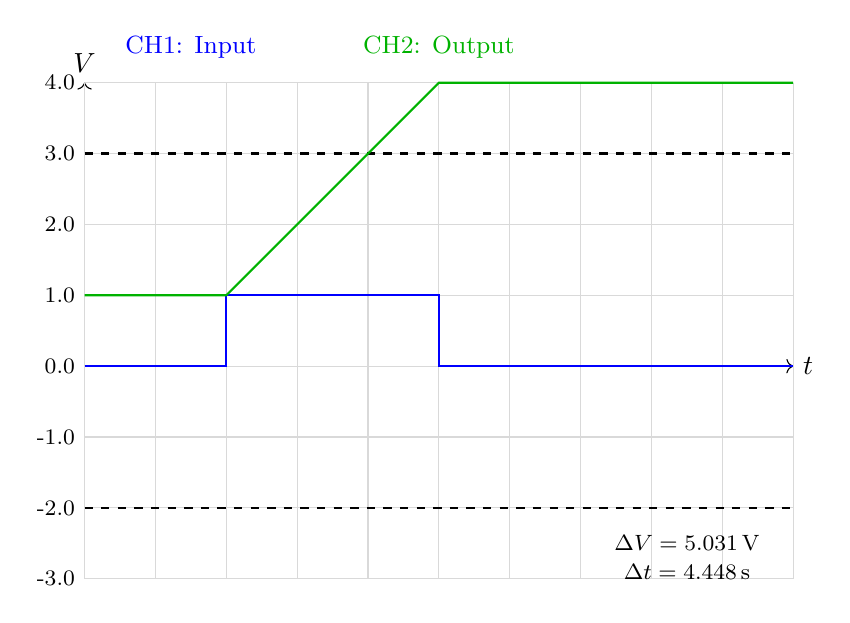
\begin{tikzpicture}[scale=0.9]
        % Draw axes
        \draw[->] (0,0) -- (10,0) node[right] {$t$};
        \draw[->] (0,-3) -- (0,4) node[above] {$V$};
        
        % Grid (light gray)
        \foreach \x in {0,1,...,10} {
            \draw[gray!30] (\x,-3) -- (\x,4);
        }
        \foreach \y in {-3,-2,-1,0,1,2,3,4} {
            \draw[gray!30] (0,\y) -- (10,\y);
        }
        
        % Y-axis labels
        \foreach \y in {-3,-2,-1,0,1,2,3,4} {
            \node[left,font=\footnotesize] at (0,\y) {\y.0};
        }
        
        % Horizontal reference lines (dashed)
        \draw[dashed,thick] (0,3) -- (10,3);
        \draw[dashed,thick] (0,-2) -- (10,-2);
        
        % Input square wave (blue, CH6 style)
        \draw[blue,thick] (0,0) -- (2,0) -- (2,1) -- (5,1) -- (5,0) -- (10,0);
        
        % Output integrated ramp (green, CH2 style)
        % When input is 1V (from t=2 to t=5), output ramps up with slope 1/RC = 1/0.5 = 2
        % From V=1 at t=2, slope=2, so at t=5 (delta_t=3), V_out = 1 + 2*3 = 7 (but clamp to 4)
        \draw[green!70!black,thick] 
            (0,1) -- (2,1)  % constant at 1V
            -- (5,4)        % ramp up (slope=2)
            -- (10,4);      % hold at saturation
        
        % Channel labels (top)
        \node[blue,above] at (1.5,4.2) {\small CH1: Input};
        \node[green!70!black,above] at (5,4.2) {\small CH2: Output};
        
        % Time and voltage delta annotation (bottom right, like in the reference)
        \node[align=left,font=\footnotesize] at (8.5,-2.5) {$\Delta V = 5.031\,\text{V}$};
        \node[align=left,font=\footnotesize] at (8.5,-2.9) {$\Delta t = 4.448\,\text{s}$};
        
    \end{tikzpicture}
    \caption{时间常数 $\tau=0.5$ 时的响应曲线}
\end{figure}
\subsubsection{PI控制器}
更进一步地,我们可以结合前面提及的比例放大器,设计出比例-积分放大器,
也就是工程中常用的PI控制器。通过添加一个输出限幅部分,
它可以满足大多数的控制需求,同时也可以比较粗糙地避免过调发生。

PI控制器的传递函数可以写为:
\begin{equation}
    G_{PI}(s) = K_p + \frac{K_i}{s} = K_p\left(1 + \frac{1}{T_i s}\right)
\end{equation}
其中 $T_i = K_p/K_i$ ,为积分时间常数。在运放实现中,可以采用单运放结构:在反馈网络中将电阻和电容串联,输入端仍为电阻。此时反馈阻抗为 $Z_f = R_f + \frac{1}{sC_f}$,传递函数为:
\begin{equation}
    G_{PI}(s) = -\frac{R_f + \frac{1}{sC_f}}{R_{in}} = -\frac{R_f}{R_{in}}\left(1 + \frac{1}{sR_fC_f}\right)
\end{equation}
比较可得:$K_p = \frac{R_f}{R_{in}}$,$T_i = R_fC_f$。

为了防止积分饱和和输出超过执行器或后级电路的耐受范围,在输出端加入限幅电路。常用的限幅方案包括:
\begin{itemize}
    \item \textbf{二极管钳位}:使用稳压二极管,将输出钳制在指定范围内。
    \item \textbf{运放饱和保护}:利用运放本身的电源轨限制输出范围,如 $\pm 12V$ 供电时输出约为 $\pm 10V$。
\end{itemize}

\begin{figure}[H]
    \centering
    \begin{circuitikz}[american, scale=1.0]
        % Define op-amp position
        \draw (3,0) node[op amp] (opamp) {};
        
        % Input signal and input resistor to inverting input (-)
        \draw (opamp.-) -- ++(-1,0) coordinate(invnode)
              to[R,l=$R_{in}$] ++(-2,0) 
              to[short,-o] ++(-0.5,0) node[left]{$V_{in}$};
        
        % Non-inverting input (+) directly to ground
        \draw (opamp.+) -- ++(0,-0.8) node[ground]{};
        
        % Output 
        \draw (opamp.out) -- ++(1.5,0) coordinate(outnode);
        
        % Feedback network: Cf (capacitor first) then Rf (resistor second), in series
        \draw (outnode) |- ++(0,1.5) coordinate(fbtop);
        
        % Capacitor Cf first (closer to output)
        \draw (fbtop) to[C,l=$C_f$] ++(-2,0) coordinate(fbmid);
        
        % Resistor Rf second (closer to inverting input)
        \draw (fbmid) to[R,l_=$R_f$] (fbmid -| invnode) |- (invnode);
        
        % Limiting circuit: two series-connected Zener diodes (back-to-back) to ground
        % From Vout: D1 (cathode up, 5.1V) in series with D2 (anode up, 5.1V) to ground
        \draw (outnode) -- ++(0.8,0) coordinate(dlimit);
        
        % Upper Zener D1: cathode pointing up (normal Zener orientation for positive limiting)
        % When Vout > +5.8V: D1 breaks down (5.1V) + forward D2 (0.7V) = 5.8V
        \draw (dlimit) to[zzDo,l_=$D_1$] ++(0,1.3) coordinate(dmid);
        
        % Lower Zener D2: anode pointing up (inverted, for negative limiting)  
        % When Vout < -5.8V: forward D1 (0.7V) + D2 breaks down (5.1V) = -5.8V
        \draw (dmid) to[zzDo,l_=$D_2$,invert] ++(0,1.3) coordinate(dtop)
              node[ground,rotate=180]{};
        
        % Final output terminal
        \draw (outnode) -- ++(1.2,0) to[short,-o] ++(0.5,0) node[right]{$V_{out}$};
        
    \end{circuitikz}
    \caption{PI控制器}
\end{figure}


这类控制器也是笔者在实际控制中运用最多的控制器。相较完整的PID控制器,它的调参更为简单,且通过直接限幅,可以将输出严格限定在要求范围内。为了验证PI控制器的实际效果,笔者搭建了参数为 $K_p=1.0$、$T_i=0.5$ 的PI控制器,并输入周期性方波信号进行测试。图中展示了输入信号、比例输出、积分输出以及经限幅后的总输出波形:

\begin{figure}[H]
    \centering
    \begin{tikzpicture}[scale=0.9]
        % Draw axes
        \draw[->] (0,0) -- (10,0) node[right] {$t$};
        \draw[->] (0,-7) -- (0,7) node[above] {$V$};
        
        % Grid (light gray)
        \foreach \x in {0,1,...,10} {
            \draw[gray!30] (\x,-7) -- (\x,7);
        }
        \foreach \y in {-6,-5,-4,-3,-2,-1,0,1,2,3,4,5,6} {
            \draw[gray!30] (0,\y) -- (10,\y);
        }
        
        % Y-axis labels
        \foreach \y in {-6,-4,-2,0,2,4,6} {
            \node[left,font=\footnotesize] at (0,\y) {\y.0};
        }
        
        % Horizontal reference lines for limits (dashed red) at ±5.8V
        \draw[dashed,red,thick] (0,5.8) -- (10,5.8) node[right,font=\small] {$+5.8V$};
        \draw[dashed,red,thick] (0,-5.8) -- (10,-5.8) node[right,font=\small] {$-5.8V$};
        
        % Input square wave (cyan/blue, CH1) - periodic, amplitude 2V
        \draw[cyan,thick] (0,0) -- (0.8,0) -- (0.8,2) -- (2,2) -- (2,0) -- (2.8,0) -- (2.8,2) -- (4,2) -- (4,0) -- (4.8,0) -- (4.8,2) -- (6,2) -- (6,0) -- (6.8,0) -- (6.8,2) -- (8,2) -- (8,0) -- (10,0);
        
        % Proportional output (purple/magenta, CH0) - follows input instantly, Kp=1
        \draw[magenta,thick] (0,0) -- (0.8,0) -- (0.8,2) -- (2,2) -- (2,0) -- (2.8,0) -- (2.8,2) -- (4,2) -- (4,0) -- (4.8,0) -- (4.8,2) -- (6,2) -- (6,0) -- (6.8,0) -- (6.8,2) -- (8,2) -- (8,0) -- (10,0);
        
        % Integral output (blue, CH6) - continuously accumulates during high, holds during low
        % Ki=2 (since Ti=0.5), slope = 2*2 = 4V/unit when input=2V
        % Each high period is 1.2 units, so deltaV = 4*1.2 = 4.8V per cycle
        % But scale down for visibility: use ~1.5V increment per cycle
        \draw[blue!70!black,thick] 
            (0,0) -- (0.8,0)      % initial low
            -- (2,1.8)            % ramp up in 1st cycle
            -- (2.8,1.8)          % hold
            -- (4,3.6)            % ramp up in 2nd cycle (1.8+1.8)
            -- (4.8,3.6)          % hold
            -- (6,5.4)            % ramp up in 3rd cycle (3.6+1.8)
            -- (6.8,5.4)          % hold
            -- (8,6)              % ramp up in 4th cycle (would be 7.2 but limit growth)
            -- (10,6);            % hold
        
        % PI output with limiting (green, CH2)
        % PI = P + I, clamped at ±5.8V
        \draw[green!70!black,very thick] 
            (0,0) -- (0.8,0)      % initial zero
            -- (0.8,2)            % instant jump (P=2V)
            -- (2,3.8)            % ramp up (P+I=2+1.8=3.8)
            -- (2,1.8)            % drop to I only
            -- (2.8,1.8)          % hold
            -- (2.8,3.8)          % jump (P=2 added)
            -- (4,5.4)            % ramp up (P+I=2+3.6=5.6)
            -- (4,3.6)            % drop to I only
            -- (4.8,3.6)          % hold
            -- (4.8,5.4)          % jump (P=2 added, 2+3.6=5.6)
            -- (5.6,5.8)          % ramp to limit
            -- (6,5.8)            % clamped at +5.8V
            -- (6,5.4)            % drop to I (but I=5.4)
            -- (6.8,5.4)          % hold
            -- (6.8,5.8)          % jump would be 7.4, clamped
            -- (8,5.8)            % stay clamped
            -- (8,5.8)            % drop but I>5.8 so still clamped
            -- (10,5.8);          % remain clamped
        
        % Channel labels (top)
        \node[cyan,above] at (1.5,6.6) {\small CH1: Input};
        \node[magenta,above] at (3.5,6.6) {\small CH0: P};
        \node[blue!70!black,above] at (5.5,6.6) {\small CH6: I};
        \node[green!70!black,above] at (8.0,6.6) {\small CH2: PI Output};
        
        % Annotation (bottom right)
        \node[align=left,font=\footnotesize] at (7.5,-6) {限幅电压: $\pm 5.8\,\text{V}$};
        \node[align=left,font=\footnotesize] at (7.5,-6.5) {$(\pm5.1V$ 稳压 $\pm 0.7V$ 导通$)$};
        
    \end{tikzpicture}
    \caption{PI控制器响应曲线 $K_p=1.0$,$T_i=0.5$,周期性方波输入,输出限幅于 $\pm 5.8V$}
\end{figure}

从波形中可以清晰地看到PI控制器的工作特性:输入方波经过比例环节得到即时响应,积分环节
则在每个高电平期间累积上升,低电平期间保持不变。两者叠加形成的PI输出在第一、二周期正常工作,但在第三周期因
积分持续累积而触发稳压二极管限幅,被钳制在 $+V_{lim}$ 附近,有效地对输出进行了限幅。当输入回到低电平时,输出立即下降,仅保留积分值。
这种限幅特性揭示了PI控制器在持续偏差输入下的积分饱和现象。

\subsection{微分环节 \texorpdfstring{\(D\)}{D} }
在运放微分器中,输入端使用电容 $C$,反馈端使用电阻 $R$。根据虚短虚断原理,流经电容的电流为:
\begin{equation}
    i(t) = C\frac{dv_i(t)}{dt}
\end{equation}
由于该电流全部流经反馈电阻 $R$,输出电压为:
\begin{equation}
    v_O(t) = -iR = -CR\frac{dv_i(t)}{dt}
\end{equation}
在频域中,传递函数为:
\begin{equation}
    \frac{V_o}{V_i} = -sCR
\end{equation}
因此微分系数为 $K_d = CR$。

\begin{figure}[H]
    \centering
    \begin{circuitikz}[american]
        % Define op-amp position
        \draw (3,0) node[op amp] (opamp) {};
        
        % Input signal and input capacitor to inverting input (-)
        \draw (opamp.-) -- ++(-1,0) coordinate(invnode)
              to[C,l=$C$] ++(-2,0) 
              to[short,-o] ++(-0.5,0) node[left]{$v_i(t)$};
        
        % Non-inverting input (+) directly to ground
        \draw (opamp.+) -- ++(0,-0.8) node[ground]{};
        
        % Output
        \draw (opamp.out) -- ++(1.5,0) coordinate(outnode) 
              to[short,-o] ++(0.5,0) node[right]{$v_O(t)$};
        
        % Feedback resistor from output to inverting input
        \draw (outnode) |- ++(0,1.5) coordinate(fbnode)
              to[R,l=$R$] (fbnode -| invnode) |- (invnode);
        

    \end{circuitikz}
    \caption{微分器}
\end{figure}
然而,纯微分器在高频时增益无限增大,会严重放大噪声。
实际应用中通常在输入端串联一个小电阻,或在反馈电阻上并联一个小电容,形成高频滚降,
使微分作用仅在有效频带内发挥。
在参数设计上,微分通道更关注有效频带与噪声抑制。通过合理选择 $R$ 和 $C$ 的值,可以在目标频段内实现微分作用。

\subsection{PID控制器设计}
综合前述的比例、积分、微分三个环节,本节将设计一个完整的模拟PID控制器。该控制器采用两级运放结构:第一级实现PID运算,第二级提供相位校正。

\subsubsection{PID控制器的传递函数}
完整的PID控制器传递函数为:
\begin{equation}
    G(s) = \frac{U_o(s)}{U_i(s)} = K_P + \frac{K_P}{T_i s} + K_P T_d s
\end{equation}

可以改写为:
\begin{equation}
    G(s) = K_P\left(1 + \frac{1}{T_i s} + T_d s\right)
\end{equation}

\subsubsection{电路结构与参数设计}
综合前文所述,PID控制器中的第一级采用如下设计:
\begin{figure}[H]
    \centering
    \begin{circuitikz}[american, scale=1.0]
        
        % Op-amp A4
        \draw (4,0) node[op amp] (opamp) {op-amp};
        
    % Input section - R0 to inverting input (add short stub for spacing)
    \draw (opamp.-) -- ++(-1,0) coordinate(inv);
    \draw (inv) -- ++(-0.5,0) coordinate(r0stub);
    \draw (r0stub) to[R,l=$R_0$] ++(-2.5,0) coordinate(rin);
    \draw (rin) to[short,-o] ++(-0.8,0) ;
        

        % Non-inverting input to ground
        \draw (opamp.+) -- ++(0,-0.8) node[ground]{};
        
        % Output - extended
        \draw (opamp.out) -- ++(2.5,0) coordinate(out);
        \draw (out) to[short,-o] ++(0.5,0) node[right,font=\small]{OUT};
        
        % Feedback network from output - extended upward
        \draw (out) -- ++(0,2.8) coordinate(fbtop);
        
        % R1 horizontal
    \draw (fbtop) to[R,l=$R_1$] ++(-2,0) coordinate(c1right);
        
        
    % At c1right, branch upward for C2-R3
    \draw (c1right) -- ++(0,0.5) coordinate(branch);
    
    % C1 horizontal (to the left)
    \draw (c1right) to[C,l=$C_1$] ++(-2,0) coordinate(c1left);
    
        % C2 vertical upward
        \draw (branch) to[C,l^=$C_2$] ++(0,1.5) coordinate(c2top);
        
        % R3 vertical upward to ground
        \draw (c2top) to[R,l^=$R_3$] ++(0,1.5) node[ground,rotate=180]{};
        
        % R2 horizontal from c1left to left
        \draw (c1left) to[R,l=$R_2$] ++(-2.5,0) coordinate(r2left);
        
    % Connect R2 back to inverting input
    \draw (r2left) |- (inv);
        
    \end{circuitikz}
    \caption{PID 单级运放电路}
\end{figure}
其中,$C_1$串联在反馈的主通路中,在低频或直流的输入信号下,其阻抗很大
而根据op-amp的特性,反馈的阻抗越大,增益越高,这正是积分控制中,对长期
存在的微小误差进行累积放大的特性。\\
而$C_2$、$R_3$支路,从直观上讲,当信号变化很慢时,电容相当于断路,信号可以直接
通过PI控制器的调整,得到输出信号;而当信号变化很快时,电容近似于导线,在结构上
相当于$R_2$、$C_1$支路被短路,也就是削弱了PI控制器的控制效果。\\
当然,上面的分析都属于只管层面的定性分析,而下文的参数计算可以提供比较科学的\\
定量分析。

\subsubsection{元器件选型}
本设计中选用的元器件规格如下表所示:

\begin{table}[H]
    \centering
    \begin{tabular}{|c|c|c|c|}
        \hline
        \textbf{元件类型} & \textbf{标号} & \textbf{参数值/型号} & \textbf{说明} \\
        \hline
        运算放大器 & U1 & LM358LV & 低压双运放,单电源或双电源供电 \\
        \hline
        输入电阻 & $R_0$ & $200\text{k}\Omega$ & 输入端串联电阻,设定输入阻抗 \\
        \hline
        反馈电阻 & $R_1$ & $100\text{k}\Omega$ & 反馈上支路电阻 \\
        \hline
        比例电阻 & $R_2$ & $100\text{k}\Omega$ & 反馈下支路电阻,决定比例系数 \\
        \hline
        微分限幅电阻 & $R_3$ & $10\text{k}\Omega$ & 限制微分增益,防止高频噪声放大 \\
        \hline
        积分电容 & $C_1$ & $1\mu\text{F}$ & 串联在反馈主路,实现积分作用 \\
        \hline
        微分电容 & $C_2$ & $1\mu\text{F}$ & 接地支路电容,实现微分作用 \\
        \hline
    \end{tabular}
    \caption{PID控制器元器件选型表}
    \label{tab:component_selection}
\end{table}

\subsubsection{参数计算}
根据电路元件值,可以计算出PID控制器的关键参数:

\textbf{积分时间常数:}
\begin{equation}
    T_i = (R_1 + R_2)C_1 = (100\text{k} + 100\text{k}) \times 1\mu\text{F} = 0.2\text{s}
\end{equation}

\textbf{微分时间常数:}
\begin{equation}
    T_d = \left(\frac{R_1R_2}{R_1+R_2} + R_3\right)C_2 = (50\text{k} + 10\text{k}) \times 1\mu\text{F} = 0.06\text{s}
\end{equation}

\textbf{比例系数:}
\begin{equation}
    K_P = \frac{R_1 + R_2}{R_0} = \frac{200\text{k}}{200\text{k}} = 1.0
\end{equation}

\textbf{微分系数:}
\begin{equation}
    K_D = \frac{(R_1 \parallel R_2) + R_3}{R_3} = \frac{50\text{k} + 10\text{k}}{10\text{k}} = 6.0
\end{equation}

\textbf{惯性时间常数:}
\begin{equation}
    \tau = R_3C_2 = 10\text{k} \times 1\mu\text{F} = 0.01\text{s}
\end{equation}

由此可得:$T_d = K_D \times \tau = 6.0 \times 0.01 = 0.06\text{s}$

\subsubsection{PSpice仿真验证}

为验证上述参数计算的正确性,使用PSpice对设计的PID控制器进行了瞬态分析仿真。输入信号为周期1秒、幅值0.5V的方波信号,仿真时间为2秒。图\ref{fig:pid_tikz}展示了输入信号与输出信号的时域响应曲线。

\begin{figure}[H]
    \centering
    \begin{tikzpicture}
    \begin{axis}[
        width=0.9\textwidth,
        height=7cm,
        xlabel={时间 (s)},
        ylabel={电压 (V)},
        grid=both,
        grid style={line width=.1pt, draw=gray!20},
        major grid style={line width=.2pt,draw=gray!50},
        legend pos=north east,
        xmin=0, xmax=0.6,
        ymin=-2, ymax=4.5,
        legend style={font=\small},
        tick label style={font=\small}
    ]
    
    % 输入信号 V(R1:1) - 方波
    \addplot[red, thick, mark=square*, mark size=1.5pt, mark repeat=10] coordinates {
        (0, 0) (0.29999, 0) (0.30001, 0.5) (0.59999, 0.5) (0.60001, 0)
    };
    \addlegendentry{输入信号 V(IN)}
    
    % 输出信号 V(U2:OUT) - 精确采样(0-0.6s)
    \addplot[green!70!black, very thick, mark=none] coordinates {
        (0, 0) (0.000001, 0.000567) (0.000006, 0.00922) (0.000014, 0.02144)
        (0.000028, 0.04386) (0.000049, 0.09851) (0.000088, 0.18425) (0.000139, 0.31291)
        (0.000216, 0.52003) (0.000345, 0.81239) (0.000520, 0.79036) (0.000683, 0.60074)
        (0.000852, 0.33368) (0.001032, -0.02105) (0.001251, -0.58686) (0.001598, -1.16857)
        (0.002071, -1.25292) (0.002440, -1.09419) (0.002799, -0.84380) (0.003028, -0.70913)
        (0.003622, -0.54706) (0.004625, -0.32103) (0.006455, -0.11065) (0.008657, -0.06067)
        (0.011061, -0.05223) (0.014839, -0.04524) (0.023030, -0.04458) (0.044771, -0.04267)
        (0.073760, -0.04082) (0.131737, -0.03734) (0.247692, -0.03129) (0.294040, -0.02040)
        (0.299999, -0.00502) (0.300000, 0.04191) (0.300001, 0.15516) (0.300002, 0.43811)
        (0.300003, 0.93394) (0.300005, 1.50776) (0.300007, 2.06689) (0.300011, 2.60250)
        (0.300017, 3.10525) (0.300024, 3.44618) (0.300032, 3.60604) (0.300042, 3.66630)
        (0.300053, 3.69867) (0.300077, 3.72496) (0.300095, 3.73176) (0.300105, 3.73195)
        (0.300117, 3.73092) (0.300139, 3.72887) (0.300214, 3.72103) (0.300400, 3.69870)
        (0.300648, 3.66313) (0.301144, 3.58063) (0.302135, 3.40573) (0.304118, 3.06410)
        (0.308084, 2.46685) (0.316016, 1.66095) (0.331879, 1.03960) (0.363606, 0.87831)
        (0.427059, 0.95827) (0.501489, 1.14527) (0.581489, 1.34307) (0.599999, 1.48869)
        (0.600000, 1.47561)
    };
    \addlegendentry{输出信号 V(OUT)}
    
    \end{axis}
    \end{tikzpicture}
    \caption{PID控制器输入输出对比 基于PSpice仿真导出结果绘制}
    \label{fig:pid_tikz}
\end{figure}

从仿真曲线可以观察到PID控制器的典型响应特征:

\begin{itemize}
    \item \textbf{微分作用(D)}:在输入信号每次跳变,如0.3s、0.9s、1.5s处,时,输出出现明显的尖峰脉冲,这是微分环节对输入变化率的快速响应。
    
    \item \textbf{比例作用(P)}:输入跳变后,输出迅速达到一个与输入成比例的稳态值。
    
    \item \textbf{积分作用(I)}:在输入信号保持高电平期间,如0.3s-0.6s、0.9s-1.2s区间,输出呈现明显的斜坡上升或下降趋势,这是积分环节对误差进行累积的结果。积分时间常数 $T_i=0.2$s 决定了斜坡的斜率。
    \end{itemize}

仿真结果验证了电路设计的正确性,所实现的单运放PID控制器(这里再次提示一下,笔者事实上用了两个运放,但第二个运放所在的第二级仅仅起到将输出相位还原的作用,为了方便就没有在原理图中绘出。)能够同时提供比例、积分、微分三种控制作用。

\section{结论}

本文基于模拟电路设计并实现了一个完整的PID控制器,通过理论分析、电路设计与仿真验证,展示了运放在控制系统中的实际应用。回顾整个设计过程,笔者认为该设计既有明显的优势,也存在一些需要改进的地方。

\subsection{设计优势}
首先,从实现成本来看,这套方案相当经济。整个控制器仅用两个运放加上几个电阻电容,总成本不过几块钱,相比需要编程的数字控制器或者专用PID芯片,门槛要低得多。对于一些简单的控制场景,比如温度控制、电机调速这类对精度要求不算太高的应用,这种模拟方案完全够用。

其次,响应速度是模拟电路的天然优势。运放的带宽通常在MHz级别,意味着它对输入变化的反应几乎是瞬时的,不像数字控制器还要经过采样、计算、输出这一套流程,延迟要大得多。从仿真结果也能看出来,在0.3s输入跳变时刻,输出的微分尖峰几乎是瞬间出现的,这种快速响应在某些对动态性能要求高的场合是很有价值的。

再者,调试过程相对直观。通过示波器可以直接观察到比例、积分、微分三个分量的波形,哪个环节出问题一目了然。想调整参数也很方便,换个电阻或电容就行,不用重新烧录程序。笔者在实验室搭建PI控制器时,就是通过观察波形快速找到合适的时间常数,整个过程非常高效。

\subsection{设计不足}
当然,这套设计也有比较明显的短板。最大的问题是参数固定,灵活性不足。电阻电容一旦焊接,PID参数就只能通过更换元件来调整。这在实际应用中很不便捷,固定的PID参数很难适应所有情况。虽然可以用电位器来实现连续调节,但这又会引入接触不良、阻值漂移等新问题。

其次,积分饱和的处理不够理想。从PI控制器的实验波形可以看到,当输入长时间保持高电平时,积分项会持续累积直到触发限幅,这时候控制器实际上已经失控。虽然加了稳压二极管限幅,但这只是被动保护,并不能从根本上解决积分windup的问题。数字PID可以通过抗积分饱和算法来处理,但模拟电路要实现类似功能就比较麻烦。

最后还有噪声敏感性的问题:微分环节天生对高频噪声敏感,虽然笔者在设计中通过$R_3$限制了微分增益,但效果还是有限。如果输入信号本身就比较毛刺,输出波形会很不干净。实际使用时可能需要在输入端加低通滤波,这又会牺牲一部分响应速度。


\subsection{未来改进方向}
基于上述分析,笔者认为可以从以下几个方面对设计进行改进。首先,可以考虑引入数字电位器,通过微控制器动态调整PID参数,在保留模拟电路响应快的优势的同时,获得一定的参数可调性。其次,对于积分饱和问题,可以尝试设计一个条件积分电路,当输出接近限幅时自动切断积分通路,避免过度累积。再次,可以在输入端增加可配置的滤波电路,根据实际噪声情况选择合适的滤波强度。

总的来说,这次设计让笔者对PID控制器的工作原理有了更深入的理解,也真切体会到了模拟电路在控制领域的应用价值。虽然存在一些局限性,但在成本、速度、易用性方面的优势还是很明显的。对于笔者这样习惯了软件算法的人来说,用硬件电路实现控制逻辑确实是一次很有意思的体验。

\section*{附录}

\subsection*{电路设计图}
\begin{figure}[H]
    \centering
    \includegraphics[width=0.85\textwidth]{design.png}
    \caption{PID控制器完整电路设计}
    \label{fig:circuit_design}
\end{figure}

\subsection*{仿真结果波形}
\begin{figure}[H]
    \centering
    \includegraphics[width=0.85\textwidth]{PIDresult.png}
    \caption{PID控制器仿真输出波形}
    \label{fig:simulation_result}
\end{figure}


\end{document}
